%\part*{Lezione 29/03/2021}
\subsection{Elettroscreening}\label{0329-sec-screening}
Passiamo alla trattazione\footnote{Calcolo ripreso dall'articolo Salpeter, E.E., Australian Journal of Physics, 1954, vol.7, p.373, \texttt{DOI:} \doi{10.1071/PH540373}.\articolo{Salpeter}} del fenomeno dell'elettroscreening\index{elettroscreening}: immaginiamo l'atomo come un gas con una alta densità nel centro, dove si concentrano tutte le cariche positive; questo comporta una nuvola polarizzata e di conseguenza a uno schermaggio del potenziale coulombiano da parte degli elettroni della nuvola elettronica (screening potenziale). Si ha allora una modifica nel termine di Gamow\index{picco di Gamow} $P(E)$ in $\mean{\sigma v}$:
$$U_{tot} (r) = \underbrace{\frac{Z_1Z_2e^2}{r}}_{U_{coul}} + U(r)$$
Definiamo allora alcune quantità che ci serviranno nel calcolo del contributo del termine $U(r)$:
\begin{itemize}
    \item $E_{\max{}}\gg kT$ è l'energia del picco di Gamow.
    \item $r_C$ è il \textit{classical turning point}\index{classical turning point@\textit{classical turning point}}, ovvero il raggio per cui $E_{\max{}} = Z_1Z_2e^2/r_C$.
    \item $r_n\ll r_C$ è il raggio nucleare, distanza dalla quale il potenziale attrattivo nucleare diviene maggiore della repulsione coulombiana.
    \item $a$ è la grandezza scala della distanza tra le particelle. Data $rho$ la densità del gas e $N_0$ il numero di Avogadro\index{numero di Avogadro}, definiamo $a$ come quel valore per cui:
    $$4\pi a^3\,\rho N_0 =1 \;\Rightarrow\; 4\pi a^3 \tilde{\rho} = 1$$
    Dal momento che\footnote{Se $M$ è misurata in a.m.u..} $\tilde{\rho} = 3M/4\pi a^3$, si ha $M= 1/3$ a.m.u., ovvero $a$ può essere visto come il raggio di una sfera di massa media pari a un terzo di unità di massa atomica.
    \item $R$ è il raggio della nuvola elettronica (vedremo che $R>a$ e $R\gg r_C$, altrimenti non si avrebbe lo screening).
\end{itemize}
Per capire come si modifica $P(E)$ dobbiamo studiare $E-U(r)-Z_1Z_2e^2/r$. Per $r\gg R$ ovviamente $U(r)\ll 1$ possiamo quindi approssimarlo come costante $U_0 \simeq Z_1Z_2e^2/R = E_{\max{}}\, r_C/R\ll1$.
\begin{figure}[!h]
    \centering
    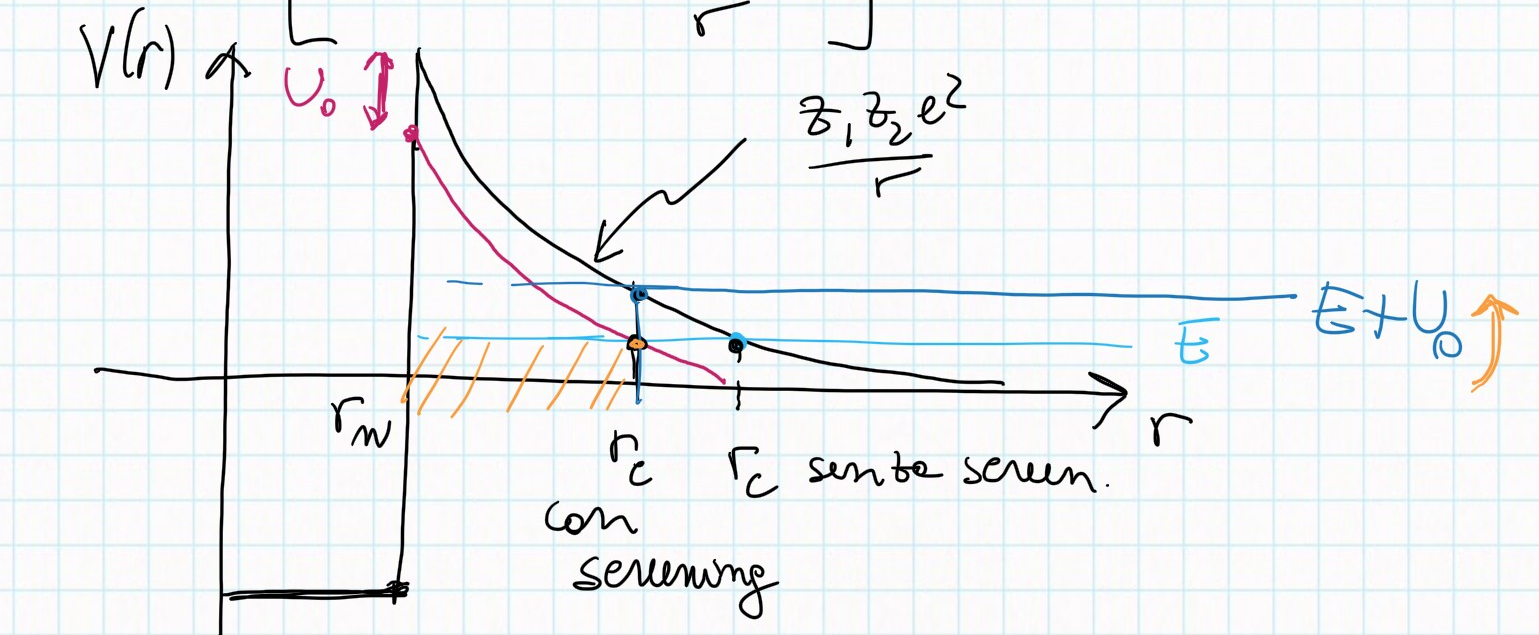
\includegraphics[scale=0.3]{Immagini/0329_pot_ES.png}
    \caption{Schema della barriera di potenziale con (linea nera) e senza (linea rosa) elettroscreening\index{elettroscreening}.}
    \label{0329_schema}
\end{figure}
\noindent Come mostrato in Figura \ref{0329_schema} l'effetto dell'elettroscreening\index{elettroscreening} è quello di abbassare la barriera di potenziale ed è possibile descrivere il problema nel caso di assenza di elettroscreening\index{elettroscreening} \textit{shiftando} l'energia $E\to E+U_0$; l'integrale allora diviene\footnote{Abbiamo approssimato l'estremo inferiore dell'integrale $U_0$ a 0, poiché $U_0/E_{\min{}}\ll1$.}:
$$\int_0^\infty dE\, S(E+U_0) P(E+U_0) e^{-(E+U_0)/kT}\: \stackrel{U_0\ll E_{\max{}}}{\simeq} e^{-U_0/kT}\PPq{\int_0^\infty dE\, S(E) P(E) e^{-E/kT}}$$
Alcuni valori tipici:
\begin{displaymath}
\begin{aligned}
r_N &\simeq 2\unit{fm} = 2\cdot\ord{-13}\unit{cm} & a   &\simeq \ord{-9}\unit{cm}\\
r_C &\simeq 2\cdot\ord{-11}\unit{cm} & R   &\simeq 3\cdot\ord{-9}\unit{cm}
\end{aligned}
\end{displaymath}
Per semplicità supponiamo che $Z_1>Z_2$ e $z\equiv Z_2$ sia la carica dei costituenti principali del gas stellare.\\ Abbiamo allora due possibili effetti:
\begin{enumerate}
    \item \textbf{screening forte}\index{elettroscreening!forte} $E_{coul} > kT$ che riguarda principalmente gli esperimenti di fusione con plasma e che anche se trattati nell'articolo di Salpeter non discuteremo.
    \item \textbf{screening debole}\index{elettroscreening!debole} $E_{coul}\ll kT$ che interessa principalmente le stelle.
\end{enumerate}

\subsubsection{Calcolo screening debole}
Ancora una volta definiamo alcune quantità utili:
\begin{itemize}
    \item[-] Il numero medio di elettroni per a.m.u. nel gas stellare: 
    $$\xi \equiv \sum_i \frac{X_iZ_i}{A_i}$$
    dove con $X_i$ si intende l'abbondanza frazionale in massa\index{abbondanza frazionale in massa}\index{fractional abundance} del nucleo $i$ con carica $Z_i$ e numero di massa $A_i$.
    \item[-] L'energia di Fermi del gas di elettroni nel caso non relativistico:
    $$E_F \equiv \frac{h^2}{8\pi^2 m^2}(3\pi^2N_0\rho\, \xi)^{2/3} = \ppc{\frac{3\pi\xi}{4}}^{2/3} \ppc{\frac{h}{a}}^2 \frac{1}{8\pi^2m^2}$$
    \item[-] Infine definiamo il rapporto:
    $$D\equiv \frac{E_F}{kT} \simeq 0.30 \frac{(\xi\rho)^{2/3}}{T_6}$$
\end{itemize}
Nel caso di screening debole\index{elettroscreening!debole} supponiamo che il gas di elettroni sia non degenere e che i costituenti principali del gas stellare abbiano $z$ e $A$; allora si ha:
$$U_{tot}(r) = Z_1 z e^2 \psi_{tot}(r)$$
$$\psi_{tot}(r) \equiv \frac{1}{r} + \psi(r)$$
Mettiamoci con $Z_1$ nel centro e con $V(r)$ potenziale elettrostatico e $\bar{\rho}(r)$ densità di carica elettronica mediati su tutte le particelle eccetto 1. Per una carica di prova $\delta Z\,e$ si ha dall'equazione di Poisson\footnote{$\nabla^2 V(r) = -4\pi{\rho}(r)$.}:
\begin{equation}\label{0329_poisson}
    \nabla^2 Z_1 e\,\psi_{tot}(r) = -4\pi\bar{\rho} -4\pi \,Z_1 e\delta^{3}(r)
\end{equation}
Per risolvere il sistema abbiamo però bisogno di un'altra equazione, che ci viene data dalla meccanica statistica:
consideriamo una regione in cui ogni particella ha energia potenziale $U_e(r)$ per cui la densità di particelle sarà data dall'espressione per la densità di particelle libere per l'esponenziale del rapporto $-U_e/kT$:
\begin{equation*}
    \bar{\rho} (r) = \underbrace{\ppc{\frac{\rho N_0ze}{A}}}_\text{densità di carica}\:\PPq{\underbrace{\exp{\ppc{-\frac{Z_1ze^2}{kT}\psi_{tot}(r)}}}_\text{parte nucleare} - \underbrace{\exp{\ppc{\frac{Z_1e^2}{kT}\psi_{tot}(r)}}}_\text{parte elettronica}}
\end{equation*}
Nel caso di screening debole possiamo sviluppare gli esponenziali al prim'ordine per cui l'espressione diviene:
\begin{equation}\label{0329_rho}
    \bar{\rho} (r) \simeq - \ppc{\frac{\rho N_0ze}{A}}\: \psi_{tot}(r) \frac{Z_1e^2}{kT} (1+z)
\end{equation}
Allora sostituendo questa in \eqref{0329_poisson} abbiamo:
$$\nabla^2 \ppc{\cancel{\frac{1}{r}} + \psi(r)} = 4\pi \rho N_0 \frac{e^2(z+z^2)}{A\, kT}  \ppc{\frac{1}{r} +\psi(r)} \cancel{-4\pi \delta^3(r)}$$
\begin{equation}\label{0329_eq}
    \nabla^2 \psi(r) = 4\pi \rho N_0 \frac{e^2(z+z^2)}{A\, kT}  \ppc{\frac{1}{r} +\psi(r)}
\end{equation}
Le condizioni al contorno per questa equazione differenziale sono imposte dalla necessità di avere il potenziale $\propto 1/r$ per grandi distanze e finito per $r=0$:
\begin{displaymath}
\begin{aligned}
&r\to +\infty & &\psi(r) \to -\frac{1}{r}\\
&r\to 0 & &\psi(r) \to \psi(0)<\infty
\end{aligned}
\end{displaymath}
Per semplicità definiamo $R_{DH}$\footnote{Dall'analisi dimensionale $[R_{DH}] = [L]$. Le lettere a pedice indicano le iniziali di Debye e \Huckel{}, questa scelta fu fatta da Salpeter poiché le soluzioni di questo problema erano le stesse di quelle della teoria delle soluzioni diluite elettrolitiche, costruita dai due scienziati\complementi{la teoria di Debye-\Huckel}.} in modo da raccogliere tutti i termini costanti in \eqref{0329_eq}:
$$R_{DH}^2 \equiv \frac{KT}{4\pi \rho N_0e^2} \frac{A}{z+z^2} = \frac{kT}{e^2} a^3$$
La soluzione è data da\footnote{$$\nabla^2 \psi(r) = \ppc{\frac{d^2}{dr^2} + \frac{2}{r}\frac{d}{dr}}\psi(r)$$}:
$$\psi(r) = \frac{1}{r}\ppc{e^{-r/R_{DH}}-1}$$
Notiamo che $\psi(0)\simeq (1-r/R_{DH}-1)/r=-1/R_{DH}$ e $\psi(r\to\infty)=-1/r$. Avremo allora per l'energia potenziale $U(r) = Z_1Z_2 e^2 \psi(r)$:
$$U(r) = Z_1Z_2 e^2 \frac{1}{r} \ppc{e^{-r/R_{DH}}-1} \qquad U(0)=U_0 = -\frac{Z_1Z_2 e^2}{R_{DH}}$$
\begin{equation}\label{0329_U0}
-\frac{U_0}{kT}\simeq 0.188 Z_1Z_2 \sqrt{\frac{\rho}{T_6^3}}\,\zeta
\end{equation}
dove abbiamo definito $\zeta\equiv \sqrt{(z+z^2)/A}$.

\paragraph{Un calcolo più preciso.}Rilassiamo a questo punto alcune delle ipotesi fatte in precedenza. Consideriamo un gas a più specie nucleari $z_i, A_i, X_i$, per cui\footnote{\acc{E} sufficiente mandare $z^2/A$ in $\sum_i X_iz^2_i/A_i$.}:
$$\bar{\rho}(r)\propto \sum_i \exp{\ppc{-Z_1 \frac{z_iX_i e^2}{kT}\psi_{tot}(r)}}$$
Inoltre dal momento che sono fermioni consideriamo gli elettroni distribuiti come una Fermi-Dirac\index{distribuzione di Fermi-Dirac}:
$$f(\eta) = \int_0^\infty dx \frac{\sqrt{x}}{e^{x-\eta}+1}$$
con $\eta \equiv \mu/kT$; per elettroni non interagenti $f(\eta) = 2D^{2/3}/3$. Poiché la densità degli elettroni si aggiusta in modo tale d uniformare il potenziale termodinamico, per elettroni interagenti avremo:
\begin{displaymath}
\begin{aligned}
f\ppc{\eta - \frac{U_e(r)}{kT}} &= \int_0^\infty dx \frac{\sqrt{x}}{e^{x-\eta}e^{U_e/kT}+1} \simeq \\
&\simeq \int_0^\infty dx \frac{\sqrt{x}}{e^{x-\eta}\ppc{1+U_e/kT}+1} =\\
&= \int_0^\infty dx \frac{\sqrt{x}}{\ppc{e^{x-\eta}+1}\ppc{1+\frac{U_e}{kT}\frac{e^{x-\eta}}{e^{x-\eta}+1}}}\simeq \\
&\simeq int_0^\infty dx \frac{\sqrt{x}}{e^{x-\eta}+1}\ppc{1-\frac{U_e}{kT}\frac{e^{x-\eta}}{e^{x-\eta}+1}} =\\
&= f(\eta) - \frac{U_e}{kT}\frac{df}{d\eta}\:\footnotemark
\end{aligned}
\end{displaymath}
\footnotetext{$$\frac{df}{d\eta} = -\int_0^\infty dx \frac{\sqrt{x}}{(e^{x-\eta}+1)^2} (-e^{x-\eta})$$}
\noindent Il rapporto tra gli elettroni interagenti e quelli non interagenti sarà dato da:
$$\frac{f(\eta-U-e/kT)}{f(\eta)} \simeq 1- \frac{U_e}{kT}\frac{f'(\eta)}{f(\eta)}$$
Questo termine entra nell'espressione di $\bar{\rho}$ influendo sul rapporto $z/A$, per cui adesso avremo la stessa espressione \eqref{0329_U0}, ma $\zeta$ sarà definito come\footnote{Ovviamente è necessario conoscere $X_i$; fino a qualche anno fa non c'erano problemi, ma negli ultimi tempi nuove misure per il Sole hanno sollevato tensioni sui valori.}:
$$\zeta \equiv \sum_i\frac{X_iz_i^2}{A_i} + \frac{f'(\eta)}{f(\eta)}\sum_i\frac{X_iz_i}{A_i}$$

\subsubsection{In laboratorio}
Studiamo allora gli effetti dell'elettroscreening\index{elettroscreening}.\\
Prendiamo un nucleo proiettile $A_1$ (per es. ioni di un nucleo) e un nucleo bersaglio $A_2$ (per es. una targhetta o un gas) per cui si ha:
$$A_1+A_2 \to A_3 + \gamma$$
Per esempio $p+\ce{^7Be}$. Dato che il nucleo è circondato dalla nuvola elettronica avremo un certo effetto di screening, tuttavia non si tratta dell'effetto di interesse astrofisico, poiché le densità stellari sono differenti da quelle ottenibili in laboratorio; non siamo quindi interessati alla sezione d'urto con lo screening ($\sigma_{lab}$), ma a quella priva di esso ($\sigma_{bare}$). Definito $\eta(E)\equiv Z_1Z_2e^2/\hbar\nu$, abbiamo dalla teoria:
$$\sigma_{lab}(E) = \frac{S(E)}{E}e^{-2\pi \eta(E)}$$
Poiché\footnote{Si tenga a mente che $U_0^{lab}\not= U_{0}^{star}$.} $U_0\ll E_{\max{}}$, detta $E_{eff}\equiv E+U_0$ si ha che $S(E)/E\approx S(E_{eff})/E_{eff}$, per cui:
$$\frac{\sigma_{lab}(E)}{\sigma_{bare}(E)} \simeq \frac{e^{-2\pi\eta(E_{eff})}}{e^{-2\pi\eta(E)}}$$
Facendo uno sviluppo per $\eta(E_{eff})$ in un intorno di $E$ e notando che $d\eta/dE = -\eta(E)/2E$ otteniamo:
$$\frac{\sigma_{lab}(E)}{\sigma_{bare}(E)} \simeq \exp{\ppc{\pi Z_1Z_2e^2 \sqrt{\frac{2\mu}{E}}\frac{U_0}{E}}}\equiv e^{g(E)}$$
Dunque per basse energie è necessario \vir{pulire} la $\sigma$ misurata secondo quell'esponenziale e poi da questa calcolarsi la $\sigma$ per i modelli stellari.\\
Solitamente $U_0\approx Z_1Z_2 e^2/R_a$ con $R_a$ raggio atomico, per cui quello che viene fatto è \textit{fittare} i dati con $U_0$ come parametro; se osserviamo per $E\to0$ un andamento crescente di tipo lorentziano abbiamo una risonanza (o stretta o sotto soglia), se invece tale andamento è $\sim \exp{(g(E))}$ allora siamo in presenza di elettroscreening\index{elettroscreening}. In ultima battuta osserviamo che minore è l'energia alla quale osserviamo e maggiore sarà la sensibilità dell'andamento a possibili effetti di screening.
